\documentclass[a4paper,landscape,10pt]{cheatsheet}

\usepackage[spanish]{babel}
\usepackage[utf8]{inputenc}
\usepackage{physics}
\usepackage{amsmath}
\usepackage{bookmark}
\usepackage{amsfonts}
\usepackage{amssymb}
\usepackage{mathtools}
\usepackage{graphicx}
\usepackage{float}
\usepackage[rightcaption]{sidecap}

%addtolength{\oddsidemargin}{.875in}
%addtolength{\evensidemargin}{.875in}
%addtolength{\textwidth}{1.75in}
%addtolength{\topmargin}{.875in}
%\addtolength{\textheight}{1.75in}

\title{Physical biology}
\author{David Caro}
\date{08-01-2024}

\pdfinfo{%
  /Title    (Physical biology)
  /Author   (David Caro)
  /Creator  (David Caro)
  /Producer (David Caro)
  /Subject  (Physics)
  /Keywords ()
}

\begin{document}
\maketitle

%%%%%%%%%%%%%%%%%%%%%%%%%%%%%%%%%%%%%%%%%%%%%%%%%%%%%%%%%%%%%%%%%%%%%%%%%
\section{1.1 Life}
Common description uses 5 characteristics:
\begin{itemize}
  \item made of cells
  \item they replicate
  \item they evolve
  \item store information (genes)
  \item use energy
\end{itemize}

\hfill\\
\section{1.2 Cellular theory}
\begin{itemize}
  \item 1665 Hook -> first microscope -> \textbf{dead cells}\\
  \item 1660-1680 Van Leeuwenhoek -> more potent microscopes -> \textbf{live cells and microorganisms}\\
  \item 1831 Brown -> \textbf{defines the nucleus}\\
  \item 1838 Schleiden (for plants), 1839 Schwann (for animals) and 1857 Virchow define the cellular theory:
        \begin{itemize}
          \item The cell is the unit of structure for life
          \item Cells retain a dual existence as individuals and building blocks
          \item (Virchow 1857) All cells come from other cells
        \end{itemize}
\end{itemize}

\hfill\\
\section{1.3 Theory of evolution}
Darwin and Wallace create the theory of evolution, two main principles:
\begin{itemize}
  \item All species are related by common ancestors.
  \item Characteristics of species change from generation to generation.
\end{itemize}
The key insight was their description of the process that pushes for that change: \textbf{natural selection}.\\
This means that you can draw a \textbf{tree of life} from the common ancestor to the current extant species.

\hfill\\
\section{1.4 Chromosomic theory of inheritance and central dogma}
Chromosomes are made of a single DNA molecule, and some of it's segments that codify the products in the cell are called genes.\\
The central dogma of microbiology states that the flow of information is unidirectional:
\begin{itemize}
  \item DNA
  \item -transcription-> mRNA
  \item -traduction-> protein
  \item -> specific trait
\end{itemize}

\hfill\\
\section{1.5 Taxonomy}
Naming organisms, started by Carl Linnaeus, binomial system, ex:\\
\begin{center}
  <gender> <species>: quercus robur (oak)
\end{center}
Added a hierarchy of taxonomical groups:\\
\begin{center}
  species < gender < family < order < class < phylum < kingdom
\end{center}
Can be drawn for all species in a phylogenetic tree, where the closest the branch, the more closely related the species.\\
Recent genetic studies have shown that this is obsolete, and currently life is classified in three domains:
\begin{itemize}
  \item Bacteria
  \item Archaea
  \item Eukarya (cells with well defined nucleus, plants, fungi, animals, ...)
\end{itemize}

\section{2.0 Biomolecules}
There's organic and inorganic molecules that are part of a living being, we will focus on the organic ones:

\hfill\\
\section*{2.1 Proteins}
Polimers of aminoacids joined by peptidic bonds, structure of an aminoacid:
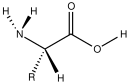
\includegraphics{images/amino_acid_structure}\\
{\footnotesize by Smokefoot - Own work, Public Domain, https://commons.wikimedia.org/w/index.php?curid=106539890}
Note the amino group $NH_2$, the acid group $COOH$, and the lateral chain with the root $R$, characteristic of every aminoacid.\\
They are joined by condensation, when the $COOH$ group creates a peptidic bind with the $NH2$ of the next.

\hfill\\
\section*{2.2 Protein structure}
There's 4 structure levels:
\begin{itemize}
  \item Primary: peptidic bonds between single aminoacids in the protein
  \item Secondary: hydrogen bonds between the $O$ of a $COOH$ group in one aminoacid and the $NH_2$ of another, can create two different shapes:
        \begin{itemize}
          \item $\alpha$-helix - $R$ groups facing outwards
          \item $\beta$-sheet
        \end{itemize}
        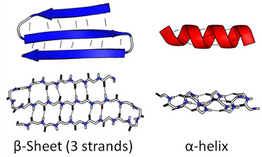
\includegraphics[width=0.2\textwidth]{images/secondary_protein_structure.png}
  \item Tertiary: \textbf{when $R$ groups are involved}, there's many kind of folds, but only a few bonds that can happen:
        \begin{itemize}
          \item \textbf{Hidrogen bonds} between $COOH$ carbonil group and the lateral chain
          \item \textbf{Hidrogen bonds} between two lateral chains or $R$ groups
          \item \textbf{Covalent bonds}, commonly di-sulfur bridge between cistein $R$ groups
          \item \textbf{Ionic bonds} between $R$ groups
          \item \textbf{Hydrophobe interactions and van der Waals forces}, when in water, the hydrophile lateral chains push
                the hydrophobe $R$ groups together, and then van der Waal forces keep them stable
        \end{itemize}
  \item Quaternary: Combination of polipeptides, bound by similar bonds than the tertiary structures.
\end{itemize}

\end{document}
